% ============================================================
% Bidang Koordinat dengan TikZ - pendamping artikel blog
% https://pakgun.gezytech.web.id/menggambar-bidang-koordinat-dengan-tikz/
% Kompilasi: pdflatex (butuh paket tikz)
% ============================================================
\documentclass{article}
\usepackage[a4paper, margin=2cm]{geometry}
\usepackage{amsmath}
\usepackage{tikz}
\usepackage{pgfplots}
\pgfplotsset{compat=1.18}

\begin{document}

\section*{1. Kanvas: petak dan dua sumbu}

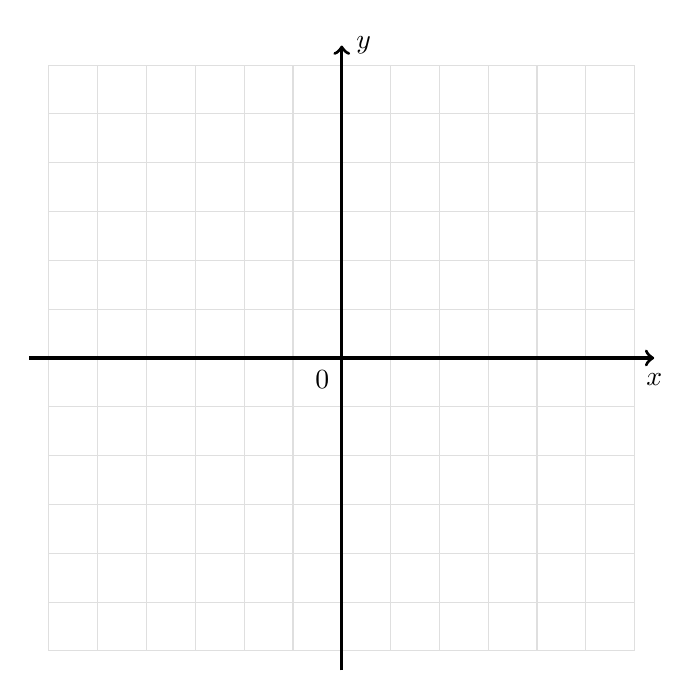
\begin{tikzpicture}[scale=0.62]
  % petak pembantu
  \draw[gray!25] (-6,-6) grid (6,6);
  % kedua sumbu
  \draw[->, very thick] (-6.4,0) -- (6.4,0);
  \draw[->, very thick] (0,-6.4) -- (0,6.4);
  \node at (6.4,-0.45) {$x$};
  \node at (0.45,6.4) {$y$};
  \node at (-0.4,-0.45) {$0$};
\end{tikzpicture}

\section*{2. Kanvas lengkap dengan angka pada sumbu}

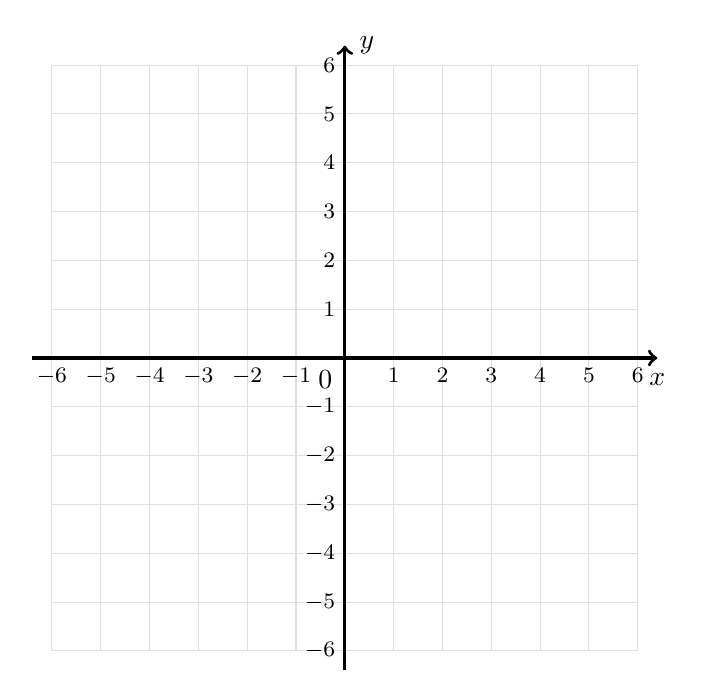
\begin{tikzpicture}[scale=0.62]
  \draw[gray!25] (-6,-6) grid (6,6);
  \draw[->, very thick] (-6.4,0) -- (6.4,0);
  \draw[->, very thick] (0,-6.4) -- (0,6.4);
  \node at (6.4,-0.45) {$x$};
  \node at (0.45,6.4) {$y$};
  \node at (-0.4,-0.45) {$0$};
  \foreach \n in {-6,...,-1,1,2,...,6} {
    \node[below] at (\n,0) {\footnotesize $\n$};
    \node[left]  at (0,\n) {\footnotesize $\n$};
  }
\end{tikzpicture}

\section*{3. Menaruh titik $P(4,1)$ dan $Q(-2,5)$}

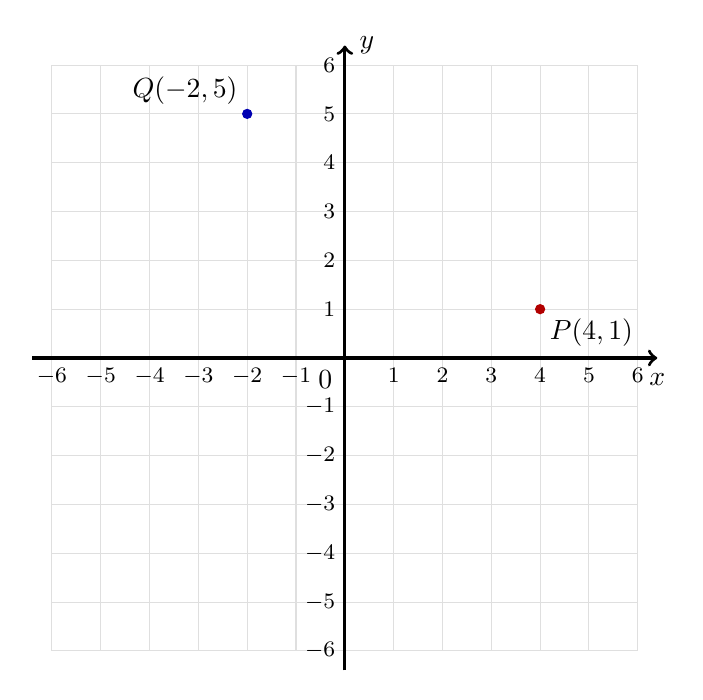
\begin{tikzpicture}[scale=0.62]
  \draw[gray!25] (-6,-6) grid (6,6);
  \draw[->, very thick] (-6.4,0) -- (6.4,0);
  \draw[->, very thick] (0,-6.4) -- (0,6.4);
  \node at (6.4,-0.45) {$x$};
  \node at (0.45,6.4) {$y$};
  \node at (-0.4,-0.45) {$0$};
  \foreach \n in {-6,...,-1,1,2,...,6} {
    \node[below] at (\n,0) {\footnotesize $\n$};
    \node[left]  at (0,\n) {\footnotesize $\n$};
  }
  \fill[red!70!black] (4,1) circle (3pt);
  \node[below right] at (4,1) {$P(4,1)$};
  \fill[blue!70!black] (-2,5) circle (3pt);
  \node[above left] at (-2,5) {$Q(-2,5)$};
\end{tikzpicture}

\section*{4. Garis melalui $P$ dan $Q$ (gradien $-\tfrac{2}{3}$)}

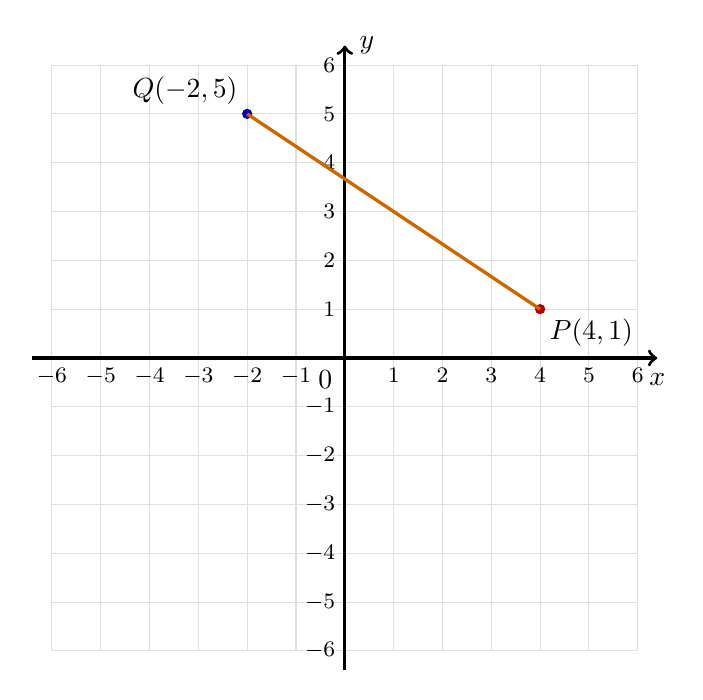
\begin{tikzpicture}[scale=0.62]
  \draw[gray!25] (-6,-6) grid (6,6);
  \draw[->, very thick] (-6.4,0) -- (6.4,0);
  \draw[->, very thick] (0,-6.4) -- (0,6.4);
  \node at (6.4,-0.45) {$x$};
  \node at (0.45,6.4) {$y$};
  \node at (-0.4,-0.45) {$0$};
  \foreach \n in {-6,...,-1,1,2,...,6} {
    \node[below] at (\n,0) {\footnotesize $\n$};
    \node[left]  at (0,\n) {\footnotesize $\n$};
  }
  \fill[red!70!black] (4,1) circle (3pt);
  \node[below right] at (4,1) {$P(4,1)$};
  \fill[blue!70!black] (-2,5) circle (3pt);
  \node[above left] at (-2,5) {$Q(-2,5)$};
  \draw[very thick, orange!80!black] (-2,5) -- (4,1);
\end{tikzpicture}

\section*{5. Cara deklaratif dengan pgfplots}

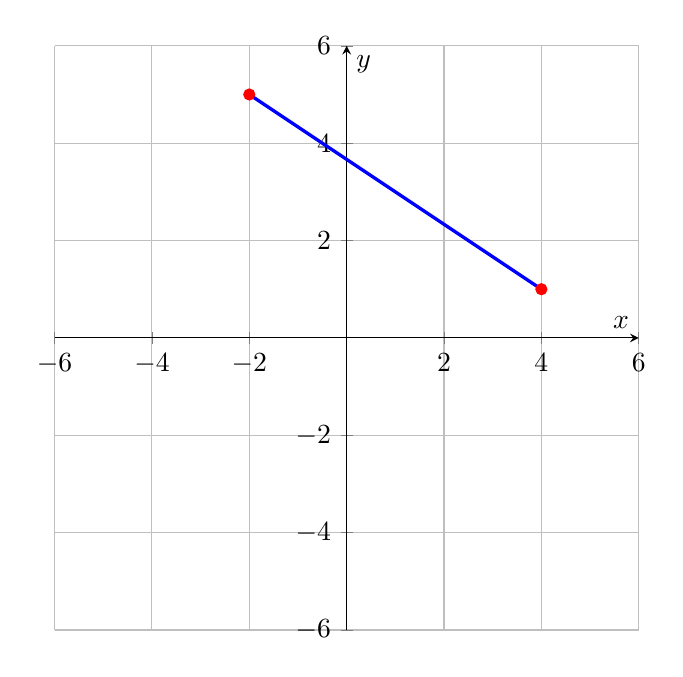
\begin{tikzpicture}
  \begin{axis}[
      axis lines = middle,
      grid = both,
      xmin = -6, xmax = 6,
      ymin = -6, ymax = 6,
      xlabel = $x$, ylabel = $y$,
      width = 9cm, height = 9cm]
    \addplot[only marks, mark = *, red]
      coordinates {(4,1) (-2,5)};
    \addplot[very thick, blue]
      coordinates {(-2,5) (4,1)};
  \end{axis}
\end{tikzpicture}

\section*{6. Contoh soal utuh: $R(5,-1)$ dan $S(-3,3)$}

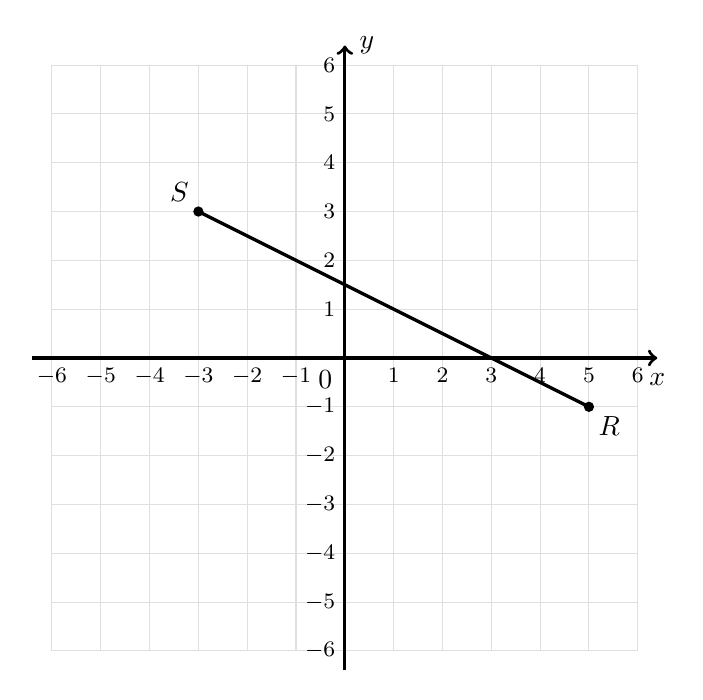
\begin{tikzpicture}[scale=0.62]
  \draw[gray!25] (-6,-6) grid (6,6);
  \draw[->, very thick] (-6.4,0) -- (6.4,0);
  \draw[->, very thick] (0,-6.4) -- (0,6.4);
  \node at (6.4,-0.45) {$x$};
  \node at (0.45,6.4) {$y$};
  \node at (-0.4,-0.45) {$0$};
  \foreach \n in {-6,...,-1,1,2,...,6} {
    \node[below] at (\n,0) {\footnotesize $\n$};
    \node[left]  at (0,\n) {\footnotesize $\n$};
  }
  \fill[black] (5,-1) circle (3pt) node[below right] {$R$};
  \fill[black] (-3,3) circle (3pt) node[above left] {$S$};
  \draw[very thick] (-3,3) -- (5,-1);
\end{tikzpicture}

\end{document}
